\newpage
\section{Ergebnisse}
\label{sec:ergebnisse}
%5.) Inhalt des Kapitels: „Ergebnisse und Resultate
%- Darstellung der eigenen Versuchsergebnisse in Sätzen in Kombination mit
%entsprechenden Tabellen (u.a. aus Messprotokoll) und Abbildungen bzw. grafischer
%Darstellung der Ergebnisse.
%- Alle Abbildungen und Tabellen sind durchzunummerieren (Abb. 01, …, Tabelle 01: …)
%und mit einer Bild- bzw. Tabellenunterschrift zu versehen.
%- Der Inhalt von Abbildungen, z.B. der Verlauf eines Graphen, ist jeweils im Text zu
%erläutern und kurz zu beschreiben. Beschreibung der Verläufe von Funktionen bzw.
%der Graphen im Text unter Verweis auf die Abbildung bzw. Abbildungsnummer und
%Herausarbeitung ihrer „Kernaussage“ und Ursache bzw. Hintergründe besonderer
%„Verläufe“.
%- Rechenwege mit denen die experimentellen Daten für die Auswertung bearbeitet
%wurden bzw. der Gang der Auswertung muss vollständig beschrieben und für einen
%Leser nachvollziehbar sein.

\subsection*{Tabellen der Messreihen 1 bis 4}
% Table generated by Excel2LaTeX from sheet 'Daten'
\begin{table}[h!]
	\centering
	\caption{Messwerte der Messreihe 1 für $T=\SI{303,15}{\kelvin}$}
	\resizebox{10.cm}{!}{
	\begin{tabulary}{1.0\textwidth}{C|CCC|C|C|C}
		\textbf{Nr.} & \textbf{$p_0 \, \left[\si{\kilo \pascal}\right]$} & \textbf{$p \, \left[\si{\kilo \pascal}\right]$} & \textbf{$h \, \left[\si{\meter}\right]$} & \textbf{$V \left[\si{\milli \liter}\right]$} & \textbf{$n \, \left[\si{\kilo \mol}\right]$}&\textbf{$V_m \, \left[\si{\liter \per \kilo \mol }\right]$} \\
		\hline
		1     & 1726  & 1715,59 & 0,078 & 4,0   & 2,7227E-06 & 0,87 \\
		2     & 1795  & 1783,39 & 0,087 & 3,8   & 2,6888E-06 & 0,82 \\
		3     & 1876  & 1863,06 & 0,097 & 3,6   & 2,6611E-06 & 0,78 \\
		4     & 1944  & 1929,46 & 0,109 & 3,4   & 2,6028E-06 & 0,74 \\
		5     & 2036  & 2020,12 & 0,119 & 3,2   & 2,5648E-06 & 0,69 \\
		6     & 2126  & 2108,79 & 0,129 & 3     & 2,5101E-06 & 0,65 \\
		7     & 2213  & 2194,59 & 0,138 & 2,8   & 2,4381E-06 & 0,61 \\
		8     & 2316  & 2296,12 & 0,149 & 2,6   & 2,3686E-06 & 0,56 \\
		9     & 2427  & 2406,05 & 0,157 & 2,4   & 2,2911E-06 & 0,52 \\
		10    & 2536  & 2513,32 & 0,170 & 2,2   & 2,1938E-06 & 0,48 \\
		11    & 2643  & 2619,25 & 0,178 & 2     & 2,0785E-06 & 0,43 \\
		12    & 2702  & 2676,65 & 0,190 & 1,8   & 1,9116E-06 & 0,39 \\
		13    & 2707  & 2680,72 & 0,197 & 1,6   & 1,7018E-06 & 0,35 \\
		14    & 2710  & 2681,98 & 0,210 & 1,4   & 1,4898E-06 & 0,30 \\
		15    & 2713  & 2683,65 & 0,220 & 1,2   & 1,2777E-06 & 0,26 \\
		16    & 2717  & 2686,18 & 0,231 & 1     & 1,0658E-06 & 0,22 \\
		17    & 2730  & 2698,11 & 0,239 & 0,8   & 8,5641E-07 & 0,17 \\
		18    & 2738  & 2705,31 & 0,245 & 0,7   & 7,5136E-07 & 0,15 \\
		19    & 2755  & 2721,78 & 0,249 & 0,6   & 6,4794E-07 & 0,13 \\
		20    & 2770  & 2735,98 & 0,255 & 0,5   & 5,4277E-07 & 0,11 \\
		21    & 3517  & 3482,71 & 0,257 & 0,4   & 5,5273E-07 & 0,09 \\
		22    & 4885  & 4850,05 & 0,262 & 0,35  & 6,7351E-07 & 0,08 
	\label{tab:m1}%
\end{tabulary}}
\end{table}%
\FloatBarrier
\vspace*{-5mm}
% Table generated by Excel2LaTeX from sheet 'Daten'
\begin{table}[h!]
	\centering
	\caption{Messwerte der Messreihe 2 für $T=\SI{313,15}{\kelvin}$}
	\resizebox{10.cm}{!}{
	\begin{tabulary}{1.0\textwidth}{C|CCC|C|C|C}
		\textbf{Nr.} & \textbf{$p_0 \, \left[\si{\kilo \pascal}\right]$} & \textbf{$p \, \left[\si{\kilo \pascal}\right]$} & \textbf{$h \, \left[\si{\meter}\right]$} & \textbf{$V \left[\si{\milli \liter}\right]$} & \textbf{$n \, \left[\si{\kilo \mol}\right]$}&\textbf{$V_m \, \left[\si{\liter \per \kilo \mol }\right]$} \\
		\hline
		1     & 1820  & 1809,72697 & 0,077 & 4,0   & 0,00287214 & 0,87 \\
		2     & 1896  & 1884,39281 & 0,087 & 3,8   & 0,00284111 & 0,83 \\
		3     & 1979  & 1965,79182 & 0,099 & 3,6   & 0,00280784 & 0,78 \\
		4     & 2064  & 2049,59107 & 0,108 & 3,4   & 0,00276489 & 0,74 \\
		5     & 2163  & 2147,25691 & 0,118 & 3,2   & 0,00272625 & 0,70 \\
		6     & 2260  & 2242,78934 & 0,129 & 3     & 0,00266958 & 0,65 \\
		7     & 2364  & 2345,32176 & 0,14  & 2,8   & 0,00260551 & 0,61 \\
		8     & 2480  & 2460,12102 & 0,149 & 2,6   & 0,00253783 & 0,57 \\
		9     & 2607  & 2585,78686 & 0,159 & 2,4   & 0,00246227 & 0,52 \\
		10    & 2740  & 2717,58611 & 0,168 & 2,2   & 0,00237213 & 0,48 \\
		11    & 2884  & 2859,98512 & 0,18  & 2     & 0,00226948 & 0,44 \\
		12    & 3027  & 3001,65096 & 0,19  & 1,8   & 0,00214371 & 0,39 \\
		13    & 3173  & 3146,58363 & 0,198 & 1,6   & 0,00199752 & 0,35 \\
		14    & 3313  & 3285,11606 & 0,209 & 1,4   & 0,00182478 & 0,30 \\
		15    & 3388  & 3358,7819 & 0,219 & 1,2   & 0,00159917 & 0,26 \\
		16    & 3396  & 3365,04749 & 0,232 & 1     & 0,00133513 & 0,22 \\
		17    & 3400  & 3368,11358 & 0,239 & 0,8   & 0,00106908 & 0,17 \\
		18    & 3408  & 3375,71333 & 0,242 & 0,7   & 0,00093755 & 0,15 \\
		19    & 3419  & 3385,51258 & 0,251 & 0,6   & 0,00080595 & 0,13 \\
		20    & 3451  & 3416,97892 & 0,255 & 0,5   & 0,00067787 & 0,11 \\
		21    & 4725  & 4690,31184 & 0,26  & 0,41  & 0,00076299 & 0,09 \\
		22    & 4945  & 4910,17842 & 0,261 & 0,4   & 0,00077927 & 0,09 
		\label{tab:m2}%
	\end{tabulary}}
\end{table}%
\FloatBarrier


% Table generated by Excel2LaTeX from sheet 'Daten'
\begin{table}[h!]
	\centering
	\caption{Messwerte der Messreihe 3 für $T=\SI{323,15}{\kelvin}$}
		\resizebox{10.5cm}{!}{
		\begin{tabulary}{1.0\textwidth}{C|CCC|C|C|C}
		\textbf{Nr.} & \textbf{$p_0 \, \left[\si{\kilo \pascal}\right]$} & \textbf{$p \, \left[\si{\kilo \pascal}\right]$} & \textbf{$h \, \left[\si{\meter}\right]$} & \textbf{$V \left[\si{\milli \liter}\right]$} & \textbf{$n \, \left[\si{\kilo \mol}\right]$}&\textbf{$V_m \, \left[\si{\liter \per \kilo \mol }\right]$} \\
		\hline
		1     & 1911  & 1900,72697 & 0,077 & 4,0   & 3,0166E-06 & 0,87 \\
		2     & 1995  & 1983,25939 & 0,088 & 3,8   & 2,9902E-06 & 0,83 \\
		3     & 2084  & 2070,79182 & 0,099 & 3,6   & 2,9578E-06 & 0,78 \\
		4     & 2177  & 2162,32424 & 0,11  & 3,4   & 2,917E-06 & 0,74 \\
		5     & 2281  & 2265,25691 & 0,118 & 3,2   & 2,8761E-06 & 0,70 \\
		6     & 2390  & 2372,78934 & 0,129 & 3     & 2,8243E-06 & 0,65 \\
		7     & 2507  & 2488,45518 & 0,139 & 2,8   & 2,7645E-06 & 0,61 \\
		8     & 2639  & 2619,25443 & 0,148 & 2,6   & 2,702E-06 & 0,57 \\
		9     & 2780  & 2758,65344 & 0,16  & 2,4   & 2,6269E-06 & 0,52 \\
		10    & 2934  & 2911,71953 & 0,167 & 2,2   & 2,5416E-06 & 0,48 \\
		11    & 3099  & 3075,25195 & 0,178 & 2     & 2,4403E-06 & 0,44 \\
		12    & 3286  & 3260,78438 & 0,189 & 1,8   & 2,3288E-06 & 0,39 \\
		13    & 3478  & 3451,18338 & 0,201 & 1,6   & 2,1909E-06 & 0,35 \\
		14    & 3667  & 3638,71581 & 0,212 & 1,4   & 2,0212E-06 & 0,30 \\
		15    & 3864  & 3834,38165 & 0,222 & 1,2   & 1,8256E-06 & 0,26 \\
		16    & 4028  & 3997,31432 & 0,23  & 1     & 1,586E-06 & 0,22 \\
		17    & 4150  & 4118,11358 & 0,239 & 0,8   & 1,3071E-06 & 0,17 \\
		18    & 4302  & 4268,646 & 0,25  & 0,6   & 1,0162E-06 & 0,13 \\
		19    & 4807  & 4772,8455 & 0,256 & 0,5   & 9,4685E-07 & 0,11 
		\label{tab:m3}%
	\end{tabulary}}
\end{table}%
\FloatBarrier
\vspace*{1.8cm}
% Table generated by Excel2LaTeX from sheet 'Daten'
\begin{table}[h!]
	\centering
	\caption{Messwerte der Messreihe 4 für $T=\SI{328,15}{\kelvin}$}
		\resizebox{10.5cm}{!}{
		\begin{tabulary}{1.0\textwidth}{C|CCC|C|C|C}
		\textbf{Nr.} & \textbf{$p_0 \, \left[\si{\kilo \pascal}\right]$} & \textbf{$p \, \left[\si{\kilo \pascal}\right]$} & \textbf{$h \, \left[\si{\meter}\right]$} & \textbf{$V \left[\si{\milli \liter}\right]$} & \textbf{$n \, \left[\si{\kilo \mol}\right]$}&\textbf{$V_m \, \left[\si{\liter \per \kilo \mol }\right]$} \\
		\hline
		1     & 1961  & 1950,72697 & 0,077 & 4,0   & 3,0959E-06 & 0,87 \\
		2     & 2043  & 2031,39281 & 0,087 & 3,8   & 3,0627E-06 & 0,83 \\
		3     & 2136  & 2122,92523 & 0,098 & 3,6   & 3,0323E-06 & 0,78 \\
		4     & 2232  & 2217,59107 & 0,108 & 3,4   & 2,9915E-06 & 0,74 \\
		5     & 2343  & 2327,1235 & 0,119 & 3,2   & 2,9546E-06 & 0,70 \\
		6     & 2457  & 2439,65592 & 0,13  & 3     & 2,9039E-06 & 0,65 \\
		7     & 2580  & 2561,58859 & 0,138 & 2,8   & 2,8458E-06 & 0,61 \\
		8     & 2716  & 2696,25443 & 0,148 & 2,6   & 2,7814E-06 & 0,57 \\
		9     & 2870  & 2848,78686 & 0,159 & 2,4   & 2,7127E-06 & 0,52 \\
		10    & 3034  & 3011,31928 & 0,17  & 2,2   & 2,6285E-06 & 0,48 \\
		11    & 3206  & 3181,98512 & 0,18  & 2     & 2,525E-06 & 0,44 \\
		12    & 3406  & 3380,78438 & 0,189 & 1,8   & 2,4145E-06 & 0,39 \\
		13    & 3621  & 3594,45022 & 0,199 & 1,6   & 2,2818E-06 & 0,35 \\
		14    & 3848  & 3819,84922 & 0,211 & 1,4   & 2,1218E-06 & 0,30 \\
		15    & 4079  & 4049,64848 & 0,22  & 1,2   & 1,9281E-06 & 0,26 \\
		16    & 4302  & 4271,44774 & 0,229 & 1     & 1,6948E-06 & 0,22 \\
		17    & 4401  & 4369,51382 & 0,236 & 0,9   & 1,5603E-06 & 0,20 \\
		18    & 4509  & 4476,4465 & 0,244 & 0,8   & 1,4209E-06 & 0,17 \\
		19    & 4627  & 4593,91283 & 0,248 & 0,7   & 1,2759E-06 & 0,15 \\
		20    & 4834  & 4800,51258 & 0,251 & 0,6   & 1,1428E-06 & 0,13058928 
		\label{tab:m4}%
	\end{tabulary}}
\end{table}%
\FloatBarrier

\begin{figure}[h!]
	\begin{center}
		\resizebox{0.8\textwidth}{!}{
			\begin{tikzpicture}[trim axis left, trim axis right]
			\begin{axis}[
			axis lines = left,
			width = 15cm,
			height = 11cm,
			xmin = 0,
			xmax = 4.5,
			ymin = 1500,
			ymax = 5000,
			%	ytick = {-4.5,-4,...,-1},
			%	xtick = {-10,-9,...,20},
			ylabel={Druck in \si{\kilo \pascal}},
			y label style={at={(-0.05,0.5)}},
			xlabel={Volumen in \si{\milli \liter}},
			legend style={at={(0.75,0.45)},anchor=west},
			%	y dir = reverse,
			]
			\addplot coordinates{(4,1715.593552) (3.8,1783.392808) (3.6,1863.058648) (3.4,1929.457656) (3.2,2020.123496) (3,2108.789336) (2.8,2194.588592) (2.6,2296.121016) (2.4,2406.053688) (2.2,2513.31928) (2,2619.251952) (1.8,2676.65096) (1.6,2680.717048) (1.4,2681.98264) (1.2,2683.64848) (0.999999999999999,2686.180904) (0.799999999999999,2698.113576) (0.699999999999999,2705.31308) (0.599999999999999,2721.779416) (0.499999999999999,2735.97892) (0.399999999999999,3482.712088) (0.35,4850.045008) };
			
			\addplot coordinates{(4,1809.726968) (3.8,1884.392808) (3.6,1965.791816) (3.4,2049.591072) (3.2,2147.256912) (3,2242.789336) (2.8,2345.32176) (2.6,2460.121016) (2.4,2585.786856) (2.2,2717.586112) (2,2859.98512) (1.8,3001.65096) (1.6,3146.583632) (1.4,3285.116056) (1.2,3358.781896) (0.999999999999999,3365.047488) (0.799999999999999,3368.113576) (0.7,3375.713328) (0.6,3385.512584) (0.5,3416.97892) (0.41,4690.31184) (0.4,4910.178424)};
			
			\addplot coordinates{(4,1900.726968) (3.8,1983.259392) (3.6,2070.791816) (3.4,2162.32424) (3.2,2265.256912) (3,2372.789336) (2.8,2488.455176) (2.6,2619.254432) (2.4,2758.65344) (2.2,2911.719528) (2,3075.251952) (1.8,3260.784376) (1.6,3451.183384) (1.4,3638.715808) (1.2,3834.381648) (0.999999999999999,3997.31432) (0.799999999999999,4118.113576) (0.6,4268.646) (0.5,4772.845504)};
			
			\addplot coordinates{(4,1950.726968) (3.8,2031.392808) (3.6,2122.925232) (3.4,2217.591072) (3.2,2327.123496) (3,2439.65592) (2.8,2561.588592) (2.6,2696.254432) (2.4,2848.786856) (2.2,3011.31928) (2,3181.98512) (1.8,3380.784376) (1.6,3594.450216) (1.4,3819.849224) (1.2,4049.64848) (0.999999999999999,4271.447736) (0.9,4369.513824) (0.8,4476.446496) (0.7,4593.912832) (0.6,4800.512584)};
			
			\legend{Messreihe 1: T=\SI{303,15}{\kelvin}, Messreihe 2: T=\SI{313,15}{\kelvin}, Messreihe 3: T=\SI{323,15}{\kelvin}, Messreihe 4: T=\SI{328,15}{\kelvin}};
			\end{axis}
			\end{tikzpicture}
		}
		\caption{Isothermen der Messreihen 1 bis 4 von \ce{SF6}}
		\label{dia:isotherme}
	\end{center}
\end{figure}
\FloatBarrier
\vspace*{-5mm}

\begin{figure}[h!]
	\begin{center}
		\resizebox{0.8\textwidth}{!}{
			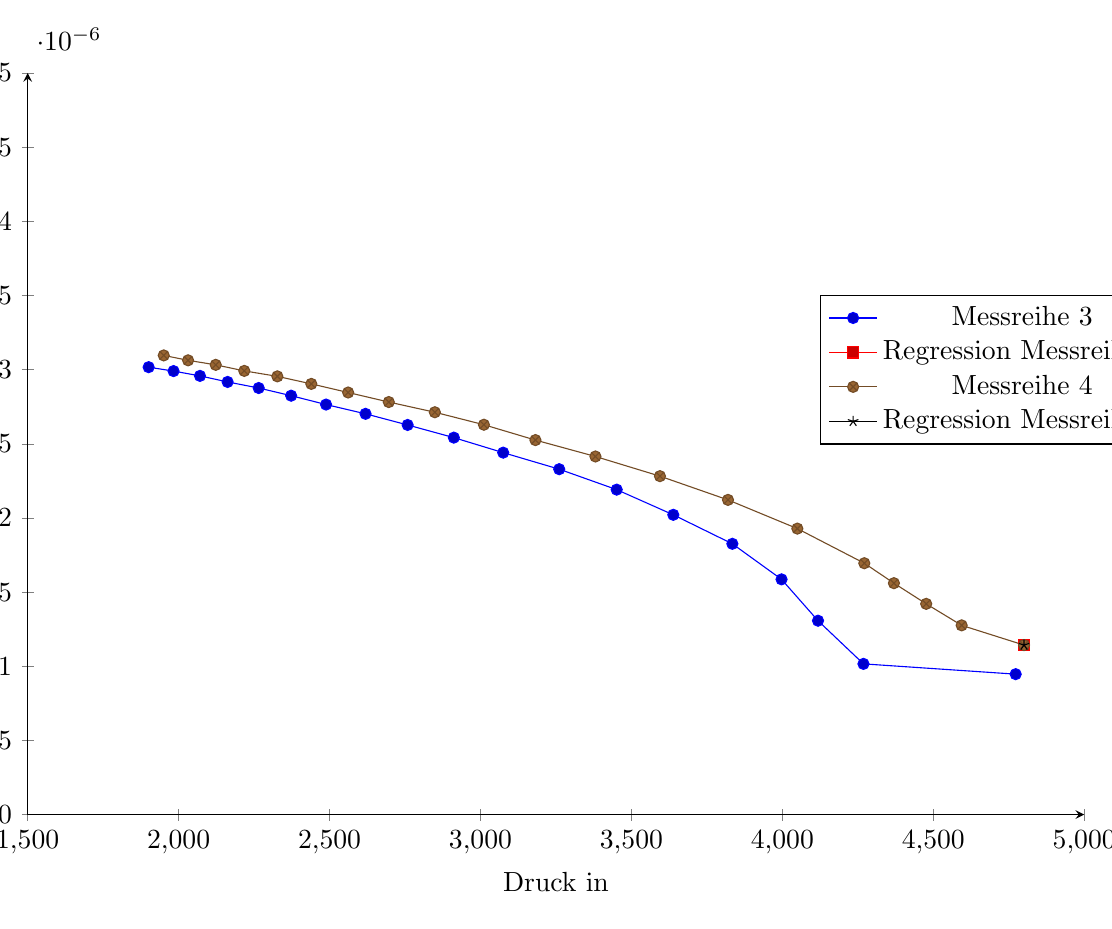
\begin{tikzpicture}[trim axis left, trim axis right]
			\begin{axis}[
			axis lines = left,
			width = 15cm,
			height = 11cm,
			xmin = 1500,
			xmax = 5000,
			ymin = 0,
			ymax = 5.e-6,
			%	ytick = {-4.5,-4,...,-1},
			%	xtick = {-10,-9,...,20},
			ylabel={Stoffmenge in \si{\kilo \mol}},
			%y label style={at={(0,0.5)}},
			xlabel={Druck in \si{\kilo \pascal}},
			legend style={at={(0.75,0.6)},anchor=west},
			%	y dir = reverse,
			]
			\addplot coordinates{(1900.726968,3.01656116192535E-06) (1983.259392,2.9901675457968E-06) (2070.791816,2.95781732177782E-06) (2162.32424,2.91697119940727E-06) (2265.256912,2.87607263434047E-06) (2372.789336,2.82431312212864E-06) (2488.455176,2.76452333998746E-06) (2619.254432,2.70198816650969E-06) (2758.65344,2.62688338717224E-06) (2911.719528,2.54158493289786E-06) (3075.251952,2.44029935853952E-06) (3260.784376,2.32877212363757E-06) (3451.183384,2.19088926166202E-06) (3638.715808,2.02119669982702E-06) (3834.381648,1.82561413934063E-06) (3997.31432,1.58599095671378E-06) (4118.113576,1.30713581518028E-06) (4268.646,1.01618738154359E-06) (4772.845504,9.46846957876465E-07) };
			
			\addplot coordinates{(4800.512584,1.14280273248285E-06)};
			
			\addplot coordinates{(1950.726968,3.09591398883609E-06) (2031.392808,3.06273847573773E-06) (2122.925232,3.03228213262785E-06) (2217.591072,2.99152604841848E-06) (2327.123496,2.95462124764783E-06) (2439.65592,2.9039039091226E-06) (2561.588592,2.84577014620481E-06) (2696.254432,2.78142034624733E-06) (2848.786856,2.7127114834769E-06) (3011.31928,2.62852367358675E-06) (3181.98512,2.5249951445989E-06) (3380.784376,2.41447317670117E-06) (3594.450216,2.28183828663598E-06) (3819.849224,2.12181084008021E-06) (4049.64848,1.92810632929653E-06) (4271.447736,1.69475726426527E-06) (4369.513824,1.56029973371969E-06) (4476.446496,1.42087473588899E-06) (4593.912832,1.27588989430243E-06) (4800.512584,1.14280273248285E-06) };
			
			\addplot coordinates{(4800.512584,1.14280273248285E-06)};
			
			\legend{Messreihe 3, Regression Messreihe 3, Messreihe 4, Regression Messreihe 4}
			\end{axis}
			\end{tikzpicture}
		}
		\caption{Berechnete Stoffmengen in Abhängigkeit vom Druck der überkritischen Messreihen 3 und 4 von \ce{SF6}}
		\label{dia:stoffmenge}
	\end{center}
\end{figure}
\FloatBarrier
\vspace*{-5mm}

\textcolor{red}{Regressionsgeraden aufstellen, Beschreibungen der Diagramme, Berechnungen der Werte }


